\documentclass{article}
\usepackage{graphicx}
\usepackage{authblk}
\usepackage[utf8]{inputenc}
\usepackage{physics}
\usepackage{parskip}
\usepackage{subcaption}
\DeclareUnicodeCharacter{2009}{\,}
\usepackage[margin=1in]{geometry}

\usepackage[
  backend=biber,
  style=chem-acs,
  articletitle=true % Optional: Set to 'true' to include article titles
]{biblatex}

\addbibresource{proposal_refs.bib}
\title{Stereo-Electronic Effects of Glycosylation}

\author[1,2]{Eugene Chung}
\affil[1]{Department of Chemistry, Hunter College, The City University of New York}
\affil[2]{The Ph.D. Program in Chemistry, The Graduate Center, The City University of New York}

\date{March 2026}
\begin{document}

\maketitle
\newpage
\begin{center}
    \Large \textbf{Committee Members}  
\end{center}
\vspace{0.5cm}

\noindent \large \textbf{Mateusz Marianski, Ph.D.} \\
Mentor, Committee Chair \\
Department of Chemistry, Hunter College, The City University of New York \\

\noindent \large \textbf{Angelo Bongiorno, Ph.D.} \\
Department of Chemistry, College of Staten Island, The City University of New York \\

\noindent \large \textbf{Mark Biscoe, Ph.D.} \\
Department of Chemistry, City College of New York, The City University of New York \\
\newpage

{\Large\bfseries Abstract}\\
\\
Glycosylation, the formation of a glycosidic bond between a sugar donor and a nucleophilic acceptor, is one of the most fundamental transformations in both synthetic chemistry and biology. It underlies the biosynthesis of glycans and Lewis antigens and enables the construction of complex carbohydrate architectures with applications ranging from vaccine development to biomaterial design. A longstanding challenge in this field is the control of stereoselectivity at the anomeric center. While the influence of C2 protecting groups on stereochemical outcomes is well established through the neighboring group effect, the extent to which remote protecting groups at C3, C4, and C6 direct selectivity remains poorly understood and actively debated. This thesis addresses two interconnected aims. The first is a systematic computational investigation of how protecting groups at each position of the sugar ring influence the stereochemical course of glycosylation, with particular emphasis on characterizing the transient oxocarbenium and dioxolenium intermediates that govern product distribution. The second aim is the development of a machine-learned potential (MLP) trained on density functional theory data, which will enable efficient and accurate ab initio-quality molecular dynamics simulations of glycosylation reactions under realistic solvation conditions. Together, these efforts will provide a unified mechanistic picture of stereo-electronic control in glycosylation and establish computational tools for the rational design of stereoselective glycosylation protocols.
\newpage
\tableofcontents
\newpage
\section{Research Aims}
\subsection{Aim 1: Identifying the Role of Protecting Groups in the Stereoslectivity of the Glycosylation Reaction}

Glycosylation can proceed through two fundamentally different substitution mechanisms, each with distinct stereochemical consequences. In an $S_N2$ pathway, departure of the leaving group and nucleophilic attack occur in a single concerted step, producing inversion of configuration at the anomeric center. The stereochemical outcome is therefore predictable: the product adopts the opposite anomeric configuration relative to the donor. In an $S_N1$ pathway, by contrast, the leaving group departs first to generate a planar oxocarbenium ion intermediate, which can then be attacked by the nucleophile from either face. It is in this latter regime that protecting groups exert their most profound influence on stereoslectivity.

The best-understood example of this influence is the neighboring group effect at C2. When a participating protecting group such as an acyl group is installed at C2, it can cyclize onto the electrophilic anomeric carbon to form a bicyclic dioxolenium ion as shown in Figure~\ref{fig:cation}. This intermediate shields one face of the anomeric center, directing nucleophilic attack to the opposite face and leading preferentially to the 1,2-\textit{trans} product (typically the $\beta$ anomer for glucopyranosides). This effect is well characterized both experimentally and computationally and serves as a reliable strategy for 1,2-\textit{trans}-selective glycosylation.

Far less understood is whether analogous participation can occur from more distant positions on the sugar ring. There is growing experimental evidence that ester protecting groups at C3, C4, and C6 can influence stereoslectivity in ways that are not easily explained by simple steric or electronic arguments. One hypothesis is that these remote groups participate directly by forming extended dioxolenium intermediates with anomeric carbon as shown in Figure~\ref{fig:cation} analogously to the effect of the neighboring group C2 but proceeding through larger and presumably less favorable ring systems. If such intermediates do form, they could account for the observed 1,2-\textit{cis} selectivity in certain glycosylation reactions a stereochemical outcome that remains one of the most significant unsolved problems in carbohydrate synthesis. 
\newpage
However, the transient nature of these putative intermediates has made their direct experimental observation exceedingly difficult.

This thesis aims to address this gap by using quantum chemical calculations to systematically map the potential energy surfaces governing glycosylation reactions with varied protecting group patterns. Specifically, the energetics and geometries of candidate dioxolenium intermediates arising from C3, C4, and C6 participation will be characterized. The goal is to determine whether these intermediates are thermodynamically and kinetically accessible, and if so, how they influence the stereochemical outcome. By comparing reactions across a matrix of protecting group identities and positions, this work will establish structure--selectivity relationships that clarify the mechanistic basis of remote group participation.
\begin{figure}[]
    \centering
    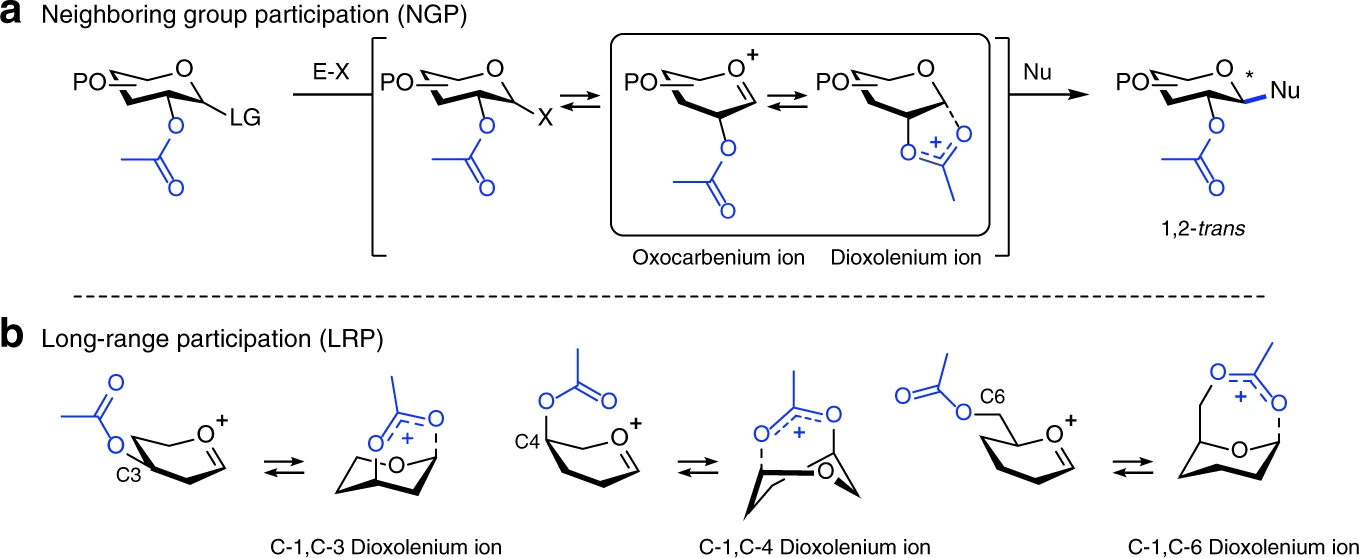
\includegraphics[width=1\linewidth]{cation.png}
    \caption{Glycosyl Cation Intermediates involving remote group participation a) Dioxolenium Ion formation in neighboring group participant b) Dioxolenium ion formation in remote group participation}
    \label{fig:cation}
\end{figure}

\subsection{Aim 2: Developing a Machine-Learned Force Field for Investigating the Stereo-Electronics of the Glycosylation Reaction via Ab Initio Molecular Dynamics}

While static quantum chemical calculations can identify key stationary points on the potential energy surface, they provide only a partial picture of a reaction that unfolds dynamically in solution. Solvent molecules play an active role in glycosylation: they stabilize charged intermediates, modulate barrier heights, and can even participate directly as nucleophiles. Capturing these effects requires molecular dynamics simulations under explicit solvation, which in turn demands energy and force evaluations at thousands of configurations along the reaction trajectory.

Ab initio molecular dynamics (AIMD) meets this requirement by computing forces from electronic structure theory at each time step, enabling the simulation of bond-forming and bond-breaking events with full quantum mechanical rigor. However, AIMD carries a severe computational cost: simulations are typically limited to a few hundred atoms and a few picoseconds of simulation time. For glycosylation reactions, where the relevant dynamics may extend over longer timescales and where adequate solvation shells require hundreds of solvent molecules, standard AIMD quickly becomes prohibitive.

Machine-learned potentials (MLPs) offer a compelling solution to this bottleneck. An MLP is a neural network trained to reproduce quantum mechanical energies and forces from a compact representation of atomic environments. Once trained, the MLP can evaluate energies and forces orders of magnitude faster than the underlying electronic structure method, while retaining near-quantum mechanical accuracy. This enables molecular dynamics simulations that combine the fidelity of AIMD with the efficiency of classical force fields.

This thesis proposes the development of an MLP specifically designed for glycosylation chemistry. The training set will be generated from DFT calculations on representative glycosyl donors, acceptors, intermediates, and transition states in explicit solvent. The resulting potential will be validated against benchmark AIMD trajectories and then deployed to perform large-scale simulations of glycosylation reactions under realistic conditions. This approach will enable a systematic, dynamics-based investigation of how protecting groups modulate the stereo-electronic landscape of glycosylation complementing and extending the static calculations of Aim 1.

\section{Background and Significance}

Understanding the stereo-electronic control of glycosylation requires tools that can accurately describe electronic structure, explore conformational and reactive landscapes, and sample dynamics under realistic conditions. This section provides the theoretical foundations for the methods employed in this thesis, beginning with the quantum mechanical framework and building toward the machine learning approaches that will enable large-scale simulations.

\subsection{Density Functional Theory}

At the heart of modern computational chemistry lies the challenge of solving the electronic Schr\"{o}dinger equation for many-electron systems a task that is analytically intractable for all but the simplest cases. Density functional theory (DFT) circumvents this difficulty by recasting the energy as a functional of the electron density, $\rho(r)$, rather than the many-body wave function. The electron density is defined as:
\begin{equation}
    \rho(r) = \sum_i g_i \braket{\psi_i(r)}{\psi_i(r)}
\end{equation}
where $g_i$ denotes the occupation number of the $i^{th}$ molecular orbital and $\psi_i(r)$ are the Kohn--Sham orbitals. The central insight of the Kohn--Sham formalism is to replace the intractable many-body problem with an auxiliary system of non-interacting electrons that reproduces the exact ground-state density. The total energy functional in the Kohn--Sham framework is expressed as:

\begin{equation}
    \varepsilon_{KS}[\rho(r)] = \int\rho(r)V_{ext}(r,R)\,dr + K[\rho(r)] + V_{ee}[\rho(r)] + \varepsilon_{XC}[\rho(r)]
\end{equation}

Each term captures a distinct physical contribution. The first term accounts for the interaction of the electrons with the external potential, $V_{ext}$, which in molecular systems arises primarily from the electrostatic attraction to the nuclei. The second term is the kinetic energy of the non-interacting reference system:
\begin{equation}
    K[\rho(r)] = -\frac{1}{2}\sum_i f_i\bra{\psi_i}\nabla^2\ket{\psi_i}
\end{equation}

The third term describes the classical electron--electron Coulomb repulsion:
\begin{equation}
    V_{ee}[\rho(r)] = \frac{1}{2}\frac{\iint\rho(r)\rho(r')\,dr\,dr'}{\abs{r-r'}}
\end{equation}

The final and most consequential term, $\varepsilon_{XC}[\rho(r)]$, is the exchange-correlation energy. This term encapsulates all quantum mechanical effects beyond the classical Coulomb interaction, including exchange arising from the Pauli exclusion principle and electron correlation. The exact form of the exchange-correlation functional is unknown, and the accuracy of any DFT calculation depends critically on the choice of approximate functional. For the chemistry of glycosylation intermediates, where non-covalent interactions and subtle conformational preferences play decisive roles, the selection of an appropriate functional is a key methodological consideration in this thesis.

\subsection{Potential Energy Surfaces}

With a method for computing molecular energies in hand, the next step is to understand how energy varies as a function of molecular geometry. This relationship is encoded in the potential energy surface (PES) a hypersurface that maps the potential energy of a system onto its internal degrees of freedom, including bond lengths, bond angles, and dihedral angles.

The PES provides the conceptual framework for understanding chemical reactivity. Reactants and products correspond to local minima on this surface, while the transition state connecting them corresponds to a first-order saddle point, a maximum along the reaction coordinate but a minimum in all orthogonal directions as shown in Figure~\ref{fig:pes}. The energy difference between the reactant and the product determines the thermodynamic driving force, while the energy barrier separating them, the activation energy, governs the rate of the reaction.
\begin{figure}[h]
    \centering
    \begin{subfigure}{0.5\linewidth}
        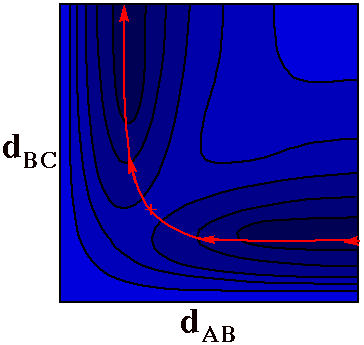
\includegraphics[width=1\linewidth]{pes.png}
    \end{subfigure}
    \begin{subfigure}{0.5\linewidth}
        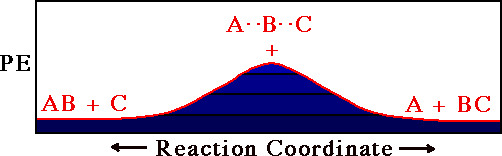
\includegraphics[width=1\linewidth]{reaction_coordinate.png}
    \end{subfigure}
    \caption{Example Potential Energy Surface with a reaction coordinate trajectory}
    \label{fig:pes}
\end{figure}

\subsection{Ab Initio Molecular Dynamics}

Static PES exploration identifies the key stationary points of a reaction, but chemistry in solution is inherently dynamic. Molecules fluctuate, solvent shells reorganize, and reactive events are stochastic. Ab initio molecular dynamics (AIMD) bridges the gap between static electronic structure calculations and the dynamic reality of chemical reactions by propagating the nuclei according to Newton's equations of motion while computing the forces at each time step from an electronic structure method such as DFT.

In contrast to classical molecular dynamics, which relies on empirical force fields with fixed functional forms, AIMD makes no assumptions about the nature of interatomic interactions. This allows it to capture phenomena that are inaccessible to classical simulations, including bond formation and cleavage, charge transfer, and changes in electronic state. For glycosylation, AIMD is uniquely suited to studying the formation and collapse of oxocarbenium and dioxolenium intermediates in the presence of explicit solvent molecules.

The principal limitation of AIMD is its computational cost. Because the electronic structure must be solved at every time step, simulations are restricted to relatively small systems (typically a few hundred atoms) and short timescales (on the order of picoseconds). For context, classical MD can routinely simulate thousands of atoms for nanoseconds or longer. This disparity motivates the development of machine-learned potentials in Aim 2, which seek to achieve AIMD-level accuracy at a fraction of the computational expense.

\subsection{Neural Networks and Machine Learning}

The machine-learned potentials at the center of Aim 2 are built upon neural network architectures, which provide the mathematical machinery for learning complex, high-dimensional mappings from data. A neural network consists of layers of interconnected computational units (neurons). Each neuron receives a weighted sum of inputs from the preceding layer, applies a nonlinear activation function, and passes the result to the next layer. The weights connecting neurons are adjustable parameters that are optimized during training.
\begin{figure}
    \centering
    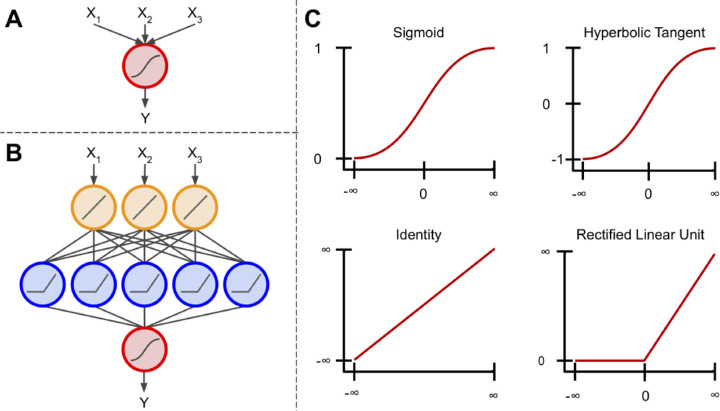
\includegraphics[width=1\linewidth]{nn.jpg}
    \caption{Overview of a neural network architecture a) The function of a single perceptron b) A graph representation of a typical neural network with the input layer in orange, hidden layer(s) in blue and output layer in red c) several commonly used functions for perceptron activation.}
    \label{fig:nn}
\end{figure}

In supervised learning, the paradigm employed here the network is trained on a dataset of input--output pairs. For an MLP, the inputs are representations of atomic configurations, and the outputs are the corresponding DFT energies and forces. During training, the network's predictions are compared to the reference data through a loss function, and the weights are iteratively adjusted to minimize this loss. The result is a model that can rapidly predict energies and forces for new, unseen configurations with an accuracy that approaches that of the underlying quantum mechanical method.

Two neural network architectures are particularly relevant to this work:

\subsubsection{Convolutional Neural Networks}
Convolutional neural networks (CNNs) are designed to exploit spatial structure in their inputs. Rather than connecting every neuron to every input, CNNs apply localized kernel filters that slide across the input tensor, detecting patterns at progressively larger scales through successive layers. The kernel elements serve as trainable parameters that are optimized during training. In the context of MLPs, CNN-like architectures can be used to process structured representations of atomic environments, capturing local geometric correlations that determine interatomic interactions.

\subsubsection{Recurrent Neural Networks}
Recurrent neural networks (RNNs) are designed for sequential data of variable length. Unlike feedforward networks, RNNs maintain a hidden state that is updated at each step of the input sequence, allowing information from earlier steps to influence the processing of later ones. This memory mechanism makes RNNs well suited for modeling time-dependent processes. In the context of this thesis, RNN architectures may prove valuable for analyzing molecular dynamics trajectories, where the temporal evolution of atomic configurations encodes mechanistic information about the glycosylation reaction.

\subsection{The Glycosylation Reaction}

With the computational toolkit established, we now turn to the chemical problem at the center of this thesis. Glycosylation is the formation of a glycosidic bond through the displacement of a leaving group at the anomeric position of a glycosyl donor by a nucleophilic acceptor. This deceptively simple definition belies the extraordinary complexity of the reaction in practice. The stereochemical outcome depends on a delicate interplay of factors: the nature of the leaving group, the identity and position of protecting groups on the sugar ring, the solvent, the temperature, and the presence of promoters or activating agents as shown in Figure~\ref{fig:factors}.

\begin{figure}
    \centering
    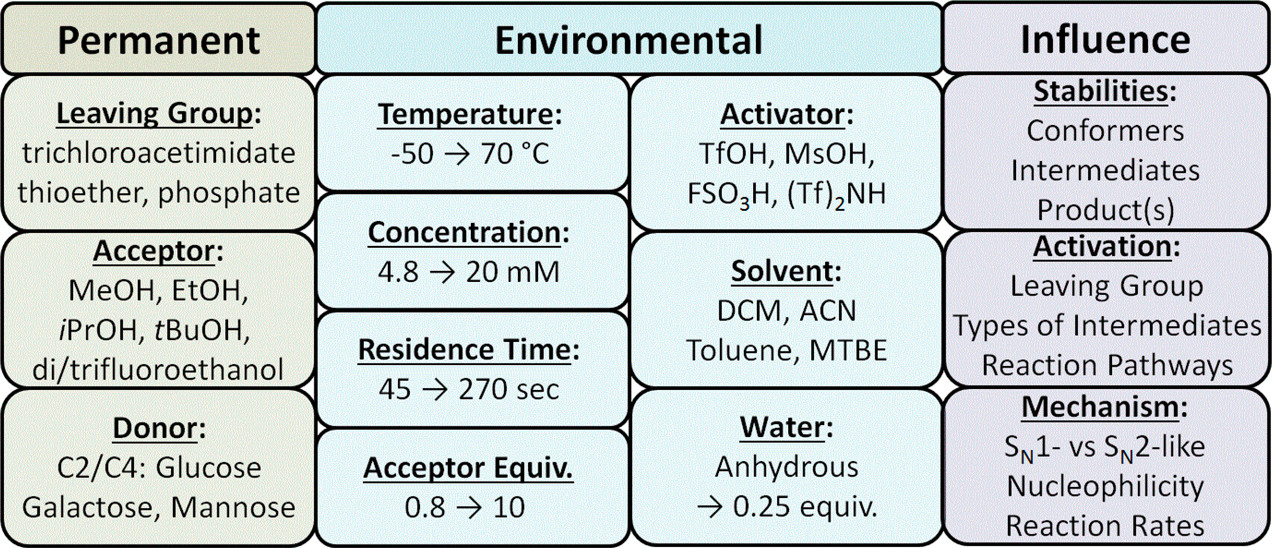
\includegraphics[width=1\linewidth]{glycosylation_factors.jpeg}
    \caption{Different factors that can alter the kinetics and selectivity of a glycosylation reaction}
    \label{fig:factors}
\end{figure}

In biological systems, glycosylation is carried out with exquisite selectivity by glycosyltransferase enzymes, producing the diverse array of glycans that decorate cell surfaces and mediate processes ranging from immune recognition to pathogen adhesion. In synthetic chemistry, achieving comparable levels of stereocontrol remains a formidable challenge. The 1,2-\textit{trans} linkage can be reliably constructed using C2 participating groups, but the stereoselective formation of 1,2-\textit{cis} linkages required for many biologically relevant glycosidic bonds lacks a general solution.

This deficiency motivates the central questions of this thesis: Can remote protecting groups at C3, C4, and C6 provide the missing element of stereocontrol? If so, what are the underlying mechanisms, and can they be predicted and optimized computationally? Answering these questions requires the combination of accurate electronic structure methods, dynamic simulations, and efficient machine learning models the integrated approach that this thesis proposes.

\section{Research Plan}
\subsection{Aim 1: Identifying the Role of Protecting Groups in the Stereoselectivity of the Glycosylation Reaction}
\subsubsection{Remote Group Participation}
The stereoselective formation of 1,2-\textit{cis}-glycosidic bonds is one of the most persistent challenges in synthetic carbohydrate chemistry. While 1,2-\textit{trans} selectivity can be achieved through C2 neighboring group participation, 1,2-\textit{cis} selectivity requires fundamentally different strategies. One of the most promising yet least understood of these is remote group participation, in which ester protecting groups at C3, C4, or C6 engage the anomeric center to form cyclic intermediates that direct the stereochemical outcome.

The mechanistic hypothesis is as follows: after departure of the leaving group, the resulting oxocarbenium ion is intercepted by the carbonyl oxygen of a remote ester group, forming a dioxolenium-type intermediate through a ring of five, six, or more atoms. This intermediate shields one face of the anomeric center, directing nucleophilic attack to the opposite face. Although this mechanism was postulated decades ago, the intermediates have never been directly observed experimentally owing to their fleeting lifetimes.

This thesis will employ DFT calculations to characterize these putative intermediates computationally. Specifically, the geometries, relative energies, and vibrational frequencies of candidate dioxolenium ions arising from C3, C4, and C6 participation will be computed for a series of model glycosyl donors. Transition states connecting the oxocarbenium ion to each dioxolenium intermediate will be located and characterized. The results will reveal whether remote participation is thermodynamically and kinetically viable, and if so, which positions and protecting group identities are most effective.

\subsubsection{Effect of Protecting Groups}
Beyond the question of whether remote groups can participate mechanistically, there is a broader need to understand how the electronic and steric properties of protecting groups at all positions of the sugar ring collectively shape the stereochemical landscape. Electron-withdrawing protecting groups are known to destabilize the oxocarbenium intermediate, potentially favoring an $S_N2$-like pathway, while electron-donating groups stabilize the cation and promote $S_N1$ chemistry. However, the interplay of these effects across multiple ring positions has not been systematically investigated.

This thesis will address this gap through a comprehensive computational survey. A matrix of glycosyl donors bearing different combinations of protecting groups at C2, C3, C4, and C6 will be studied. For each combination, the key stationary points on the glycosylation PES including reactants, oxocarbenium intermediates, dioxolenium intermediates (where applicable), transition states, and products will be computed. The resulting dataset will enable the construction of quantitative structure--selectivity relationships that map protecting group identity and position to stereochemical outcome.

\subsection{Aim 2: Machine-Learned Potentials for Glycosylation Dynamics}

The static calculations of Aim 1 will provide essential mechanistic insights, but a complete understanding of glycosylation stereoselectivity requires accounting for the dynamic and solvent-mediated aspects of the reaction. This is the objective of Aim 2, which focuses on developing and deploying machine-learned potentials for glycosylation chemistry.

The development of the MLP will proceed in several stages. First, a diverse training set will be generated by performing DFT calculations on snapshots drawn from preliminary AIMD trajectories of model glycosylation reactions in explicit solvent. This dataset will include configurations spanning reactants, intermediates, transition states, and products, ensuring that the MLP is trained across the full reactive landscape. Second, a neural network architecture will be selected and trained to reproduce the DFT energies and forces. The model will be validated by comparing its predictions to independent DFT calculations and to benchmark AIMD trajectories not included in the training set.

Once validated, the MLP will be used to perform large-scale molecular dynamics simulations of glycosylation reactions under conditions that would be computationally intractable with standard AIMD. These simulations will provide dynamical insight into the lifetimes of reactive intermediates, the role of solvent in stabilizing or destabilizing specific pathways, and the kinetic competition between different stereochemical outcomes. By systematically varying the protecting group pattern across simulations, this approach will complement the static analysis of Aim 1 and yield a comprehensive, dynamics-informed picture of stereo-electronic control in glycosylation.

\newpage
\nocite{*}
\printbibliography
\end{document}
